\subsection{Charge misassignment background}
The background from processes with prompt opposite-sign lepton pairs like \ttbar\ or DY+jets, where one of the two leptons has a wrongly assigned charge, is estimated from the measured charge misassignment probabilities and the events of a corresponding opposite-sign control region.
Naturally, this background is only relevant for the same-sign dilepton channels.
Studies in MC show the charge misassignment probability for muons to be negligible, and we subsequently restrict ourselves to electrons.

\subsubsection{Measurement of the electron charge misassignment probabilities}
The charge misassignment probability for electrons can be extracted from the data, in events with two same-sign electrons with invariant mass close to the mass of the \Z\ boson.
Electron pairs in the peak are sure to be from real opposite sign pairs with a wrongly assigned charge on one leg.
% Figure~\ref{fig:samesign_Z_peak} shows the same-sign \Z\ peak for events where exactly two good electrons pass the full selection.

% \begin{figure}[htp]
% 	\centering
% 	\includegraphics[width=0.40\textwidth]{plots_leptons/chargeflip/minMllAFAS_with_tightcharge.pdf}
% 	\includegraphics[width=0.40\textwidth]{plots_leptons/chargeflip/minMllAFAS_no_tightcharge.pdf}
% 	\caption{
% 	Di-electron invariant mass for same-sign pairs passing the full electron selection, including the triple charge agreement (left), and excluding it (right).
% 	Events in the left plot are used to extract the charge misassignment probability.
% 	}
% 	\label{fig:samesign_Z_peak}
% \end{figure}

Charge misassignment probabilities are calculated for different bins of electron \pt\ and $\eta$ by extracting same-sign and opposite-sign event yields categorized in the kinematics of the two lepton legs.
In each category, the event yield of electron pairs from \Z\ decays is determined from a fit to the invariant mass shape, and depends on the charge misassignment probabilities of each leg.
The invariant mass shape is modeled with a crystal ball and Breit-Wigner function for the signal and an exponentially falling function for the backgrounds.

Electron kinematics are separated in three \pt\ (10--25\GeV, 25--50\GeV, and $\geq$50\GeV) and two $\eta$ bins (0--1.479 and 1.479--2.5), resulting in a total of 21 distinct categories of electron pairs.
The six charge misassignment probabilities are then determined in a simultaneous fit to the 21 same-sign and opposite-sign event yields.

The resulting misassignment probabilities range between about 0.03\% in the barrel and about 0.4\% in the end caps and are shown in Tab.~\ref{tab:chmisid_prob} and Fig.~\ref{fig:chmisid_prob}.

\begin{table}[htp]
\centering
\caption{
	Electron charge misassignment probabilities (in percent) as determined in data (top) and Drell--Yan MC (bottom).
}
\label{tab:chmisid_prob}
\begin{tabular}{lccc}
	\hline
	  Data                & $10\leq\pt<25\GeV$ & $25\leq\pt<50\GeV$ & $50\GeV\leq\pt$ \\
	\hline
	 $0\leq\eta<1.479$    & 0.0442 $\pm$ 0.0011 & 0.0179 $\pm$ 0.0004 & 0.0262 $\pm$ 0.0020 \\
	 $1.479\leq\eta<2.5$  & 0.1329 $\pm$ 0.0066 & 0.1898 $\pm$ 0.0014 & 0.3067 $\pm$ 0.0113 \\
	\hline
	\hline
	  MC                  &  &  & \\
	\hline
	 $0\leq\eta<1.479$    & 0.0378 $\pm$ 0.0016 & 0.0222 $\pm$ 0.0003 & 0.0233 $\pm$ 0.0015 \\
	 $1.479\leq\eta<2.5$  & 0.0956 $\pm$ 0.0044 & 0.2108 $\pm$ 0.0027 & 0.3157 $\pm$ 0.0018 \\
	\hline
\end{tabular}
\end{table}


\begin{figure}[htp]
	\centering
	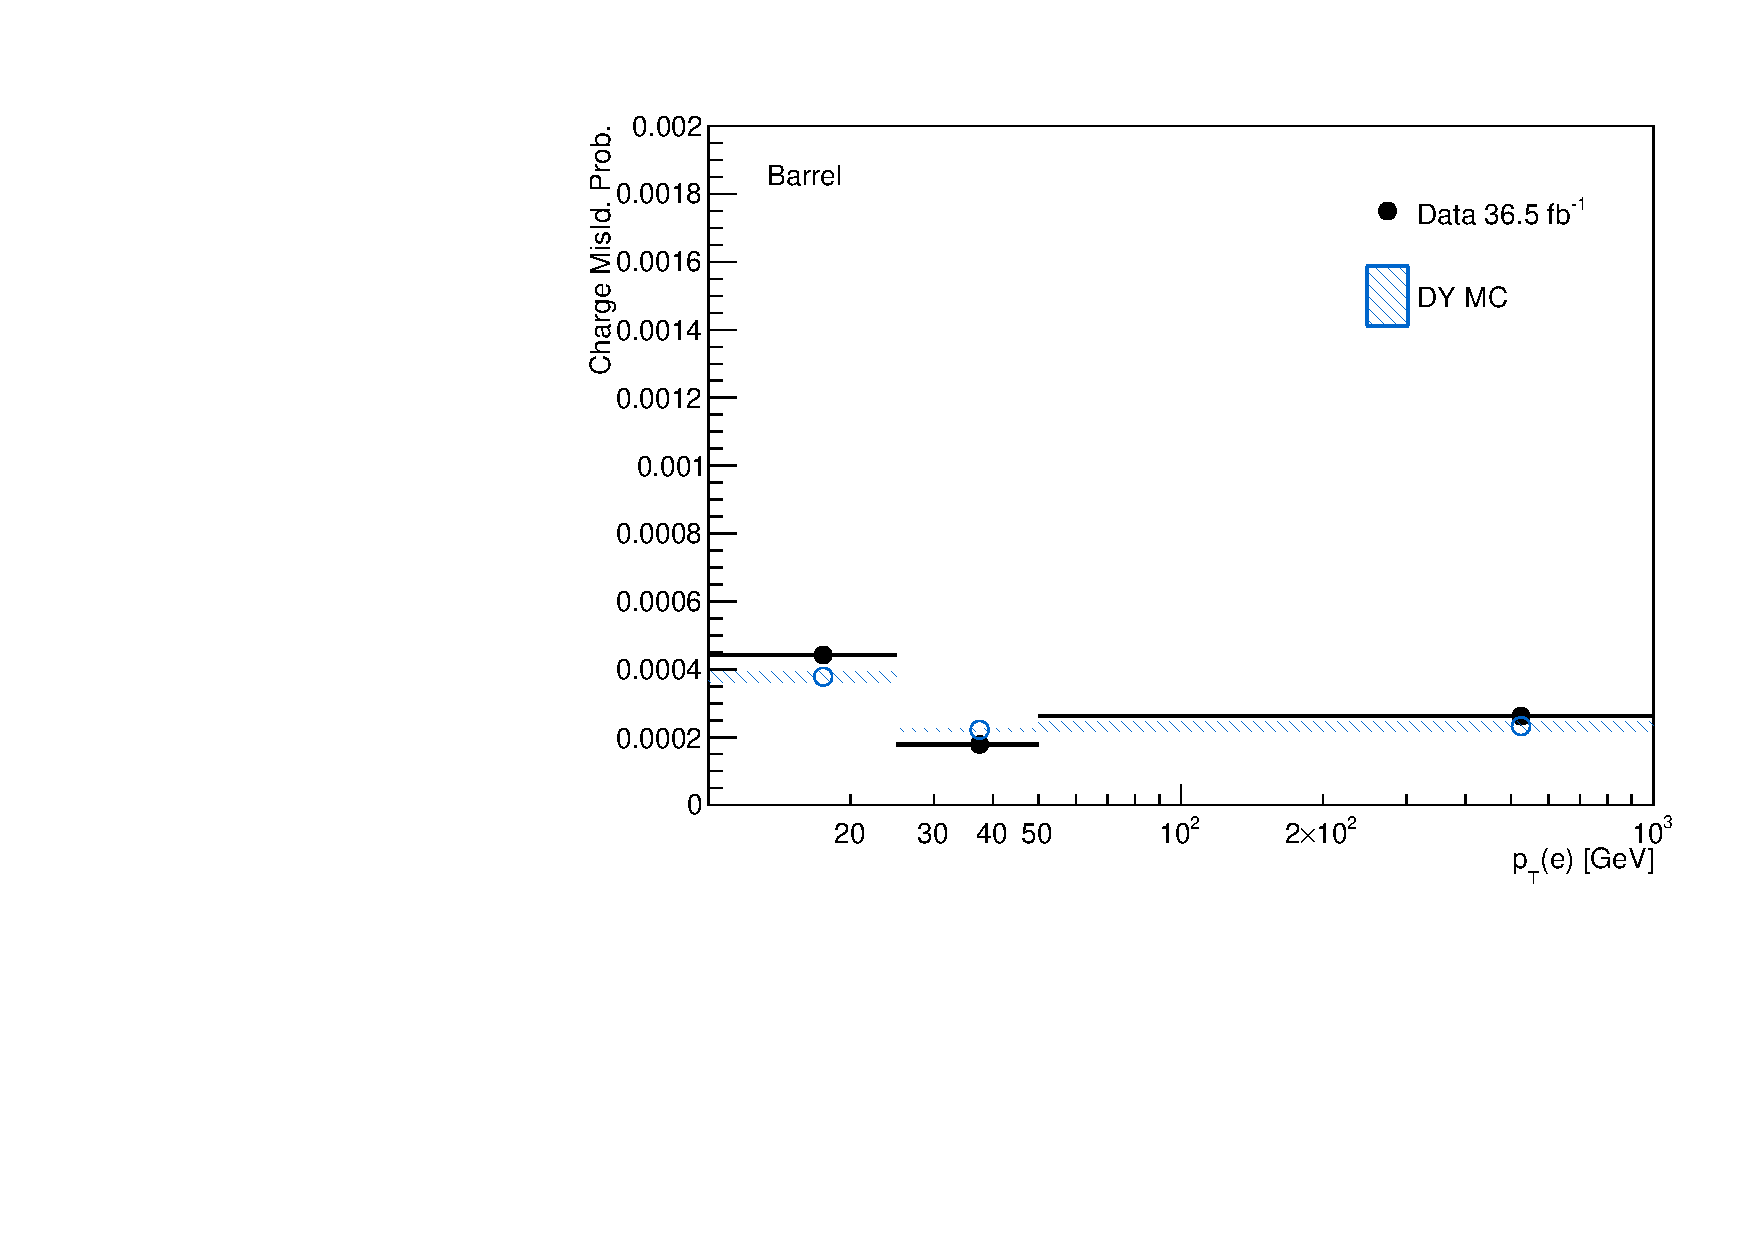
\includegraphics[width=0.49\textwidth]{plots_leptons/chargeflip/chmid_prob_barrel.pdf}
	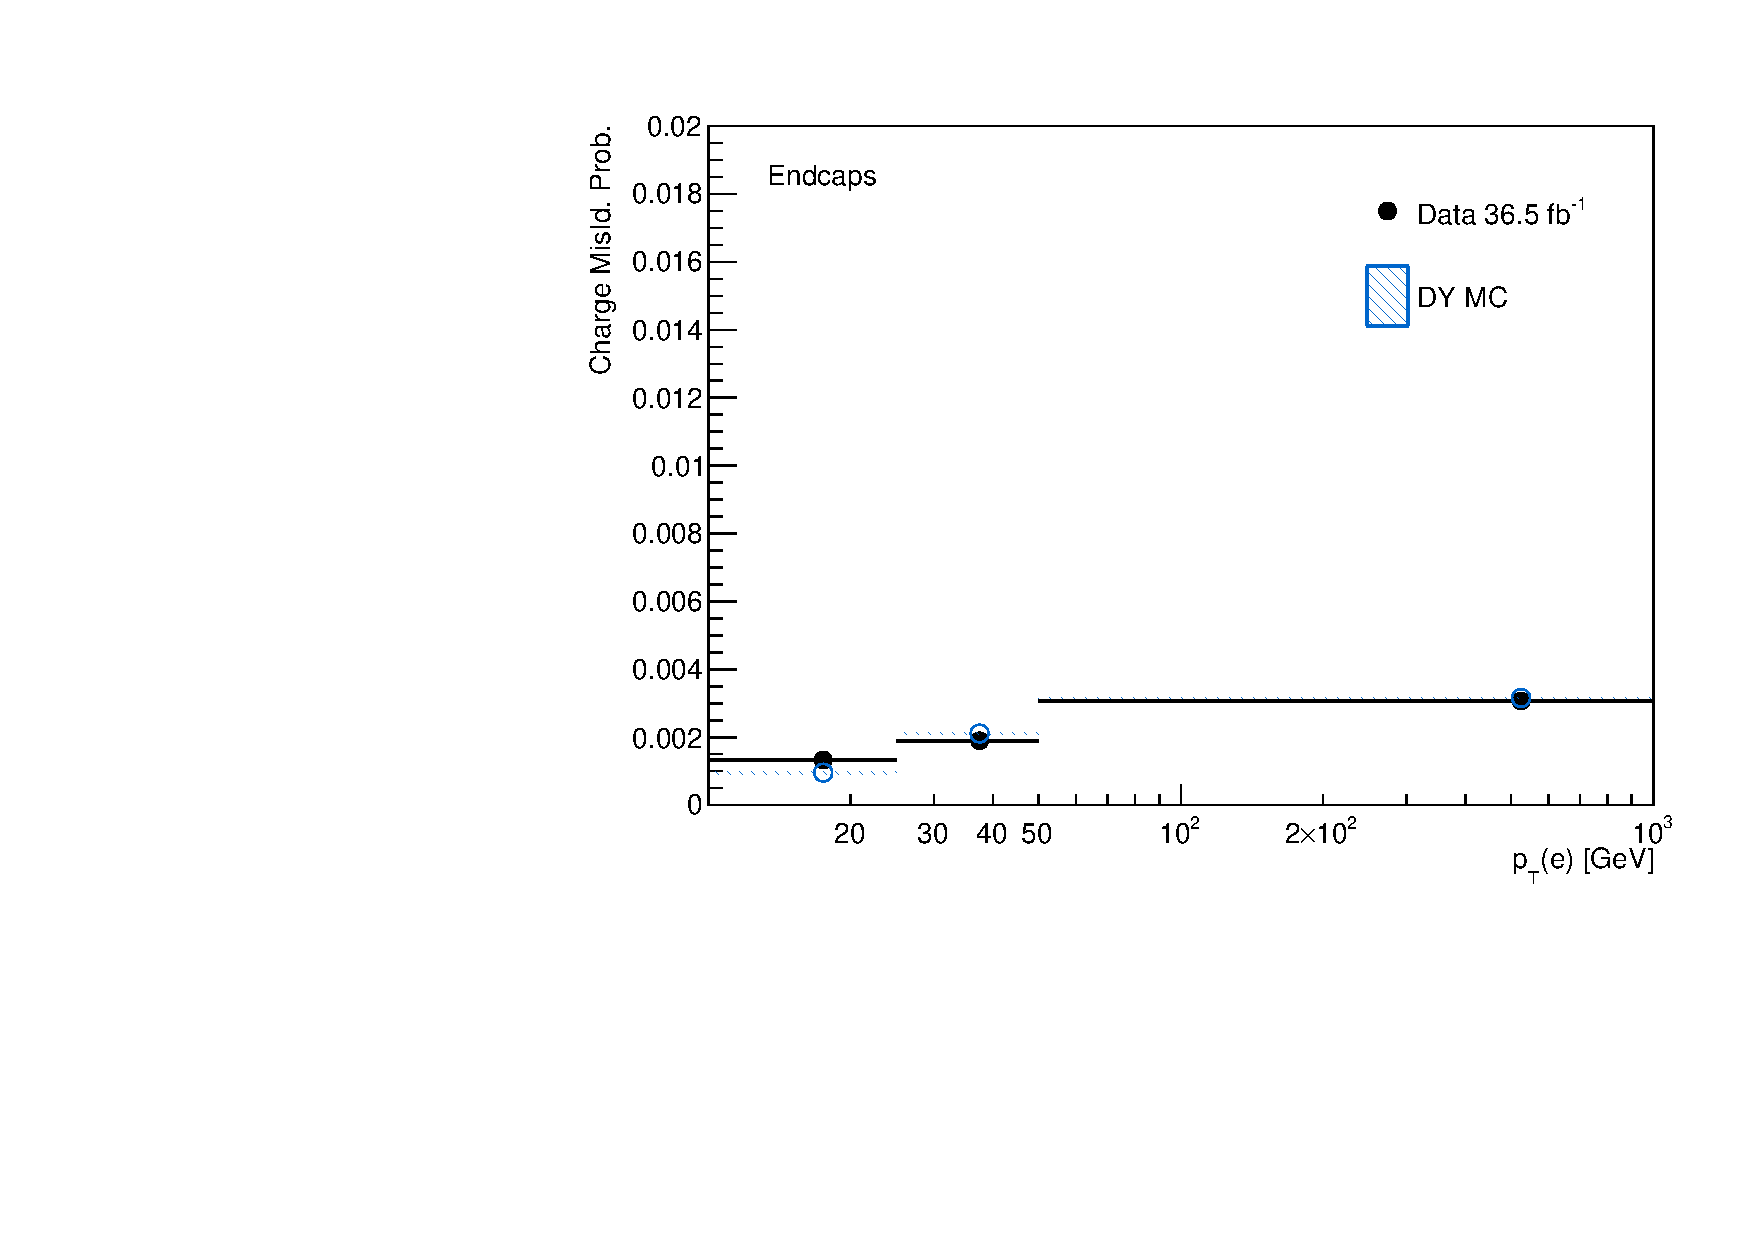
\includegraphics[width=0.49\textwidth]{plots_leptons/chargeflip/chmid_prob_endcap.pdf}
	\caption{
	Electron charge misassignment probabilities as a function of \pt\ for electrons in the barrel (left) and endcaps (right). Note the change in y-axis scale.
	}
	\label{fig:chmisid_prob}
\end{figure}


\subsubsection{Background estimation}
Contributions from opposite-sign prompt leptons with charge-misassigned electrons to the same-sign dilepton channels with electrons (ee, and e$\mu$) are then estimated from the events of a control region with identical selection except for the requirement of equal charge of the lepton pair.
Each event in the control region is assigned a weight of $P(\pt,\eta)$ for each electron with a given \pt\ and $\eta$ in the event (\ie\ ee events get a weight of $P_1+P_2$ and e$\mu$ events get a weight of $P$), where $P$ is the measured charge misassignment probability.

The procedure is tested in two control regions: once using the same events that were used to measure the probabilities, dominated by DY events, and once in a selection with at least one medium b-tagged jet or two loose b-tagged jet and between 2 and 3 hadronic jets, with a significant contribution from \ttbar\ events.
Event distributions in the two control regions where the background from charge misassigned electrons is estimated as described are shown in Fig.~\ref{fig:chmisid_closure_dy} and \ref{fig:chmisid_closure_tt}.


\begin{figure}[htp]
	\centering
	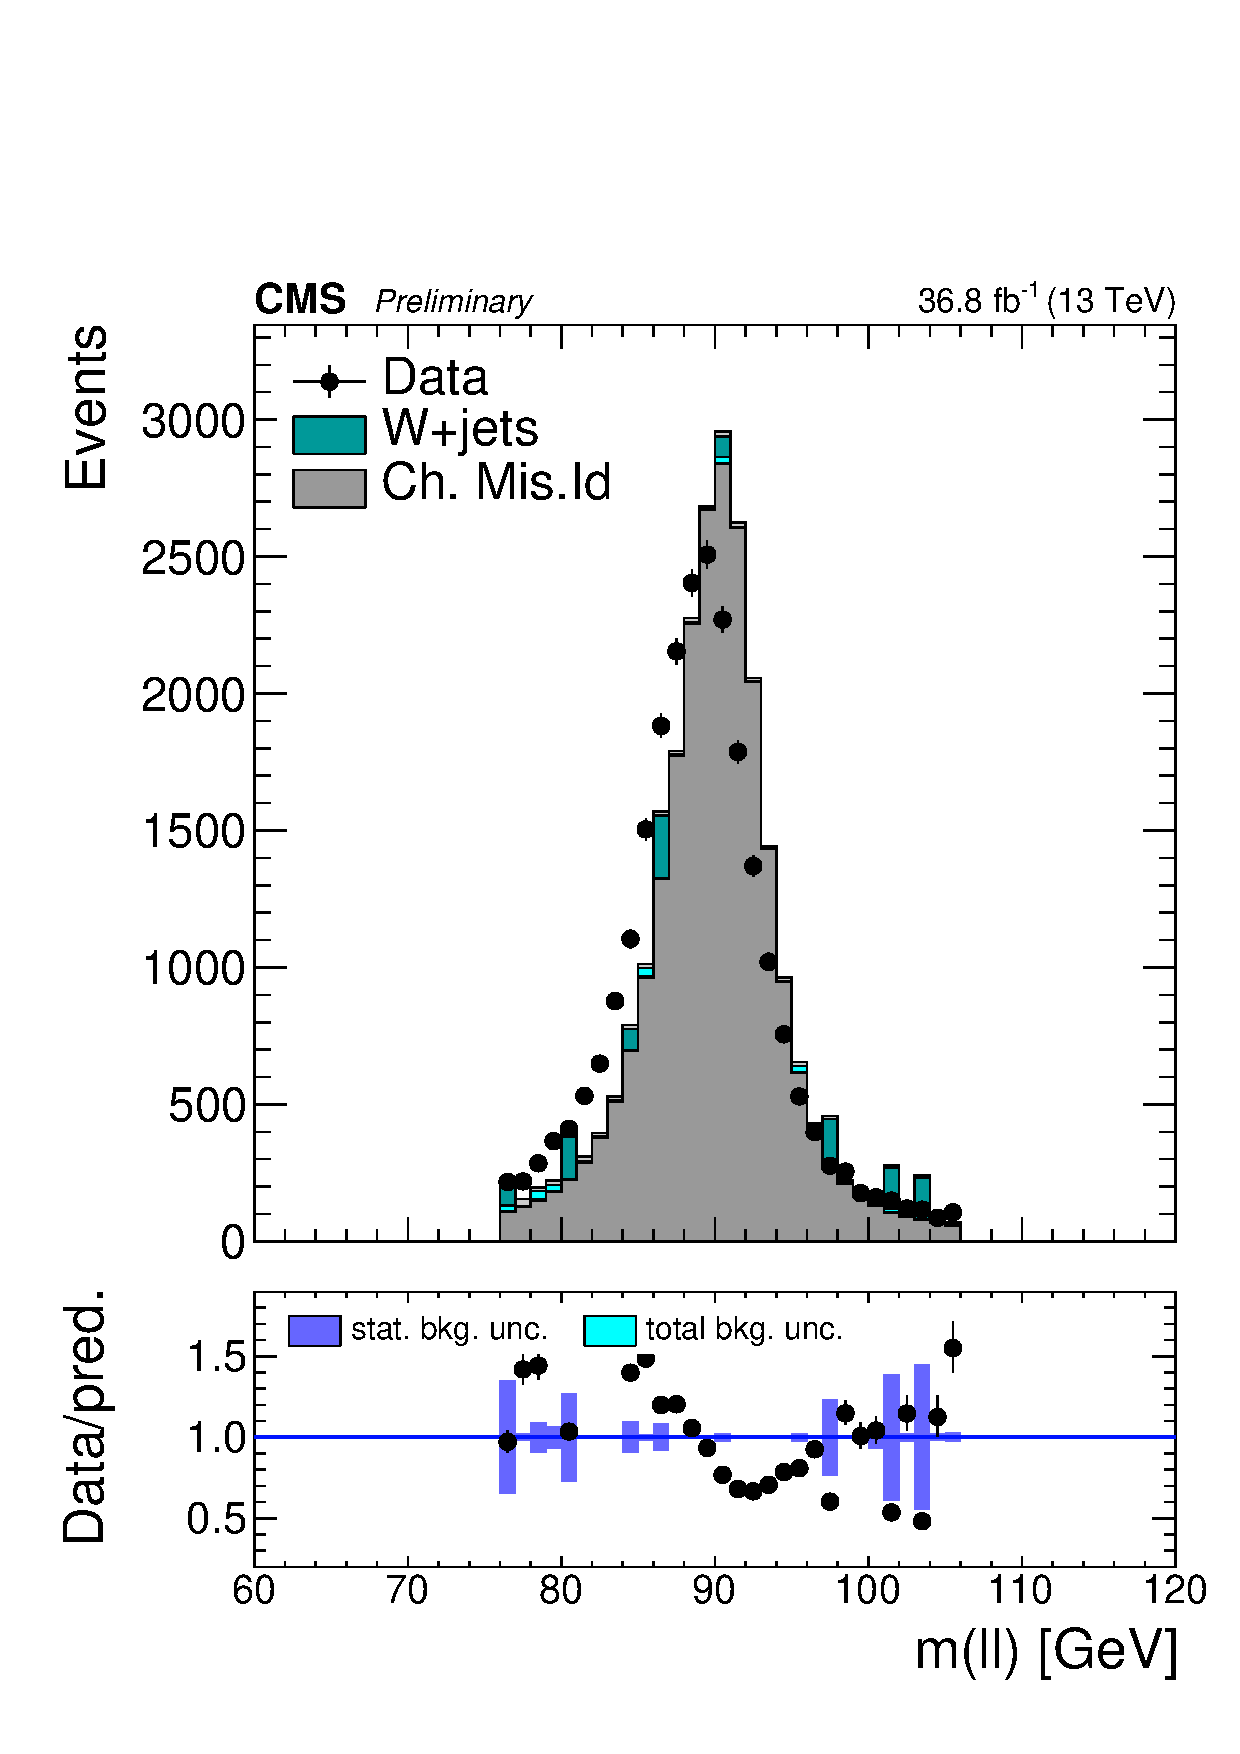
\includegraphics[width=0.32\textwidth]{plots_leptons/chargeflip/closure_dy/minMllAFAS.pdf}
	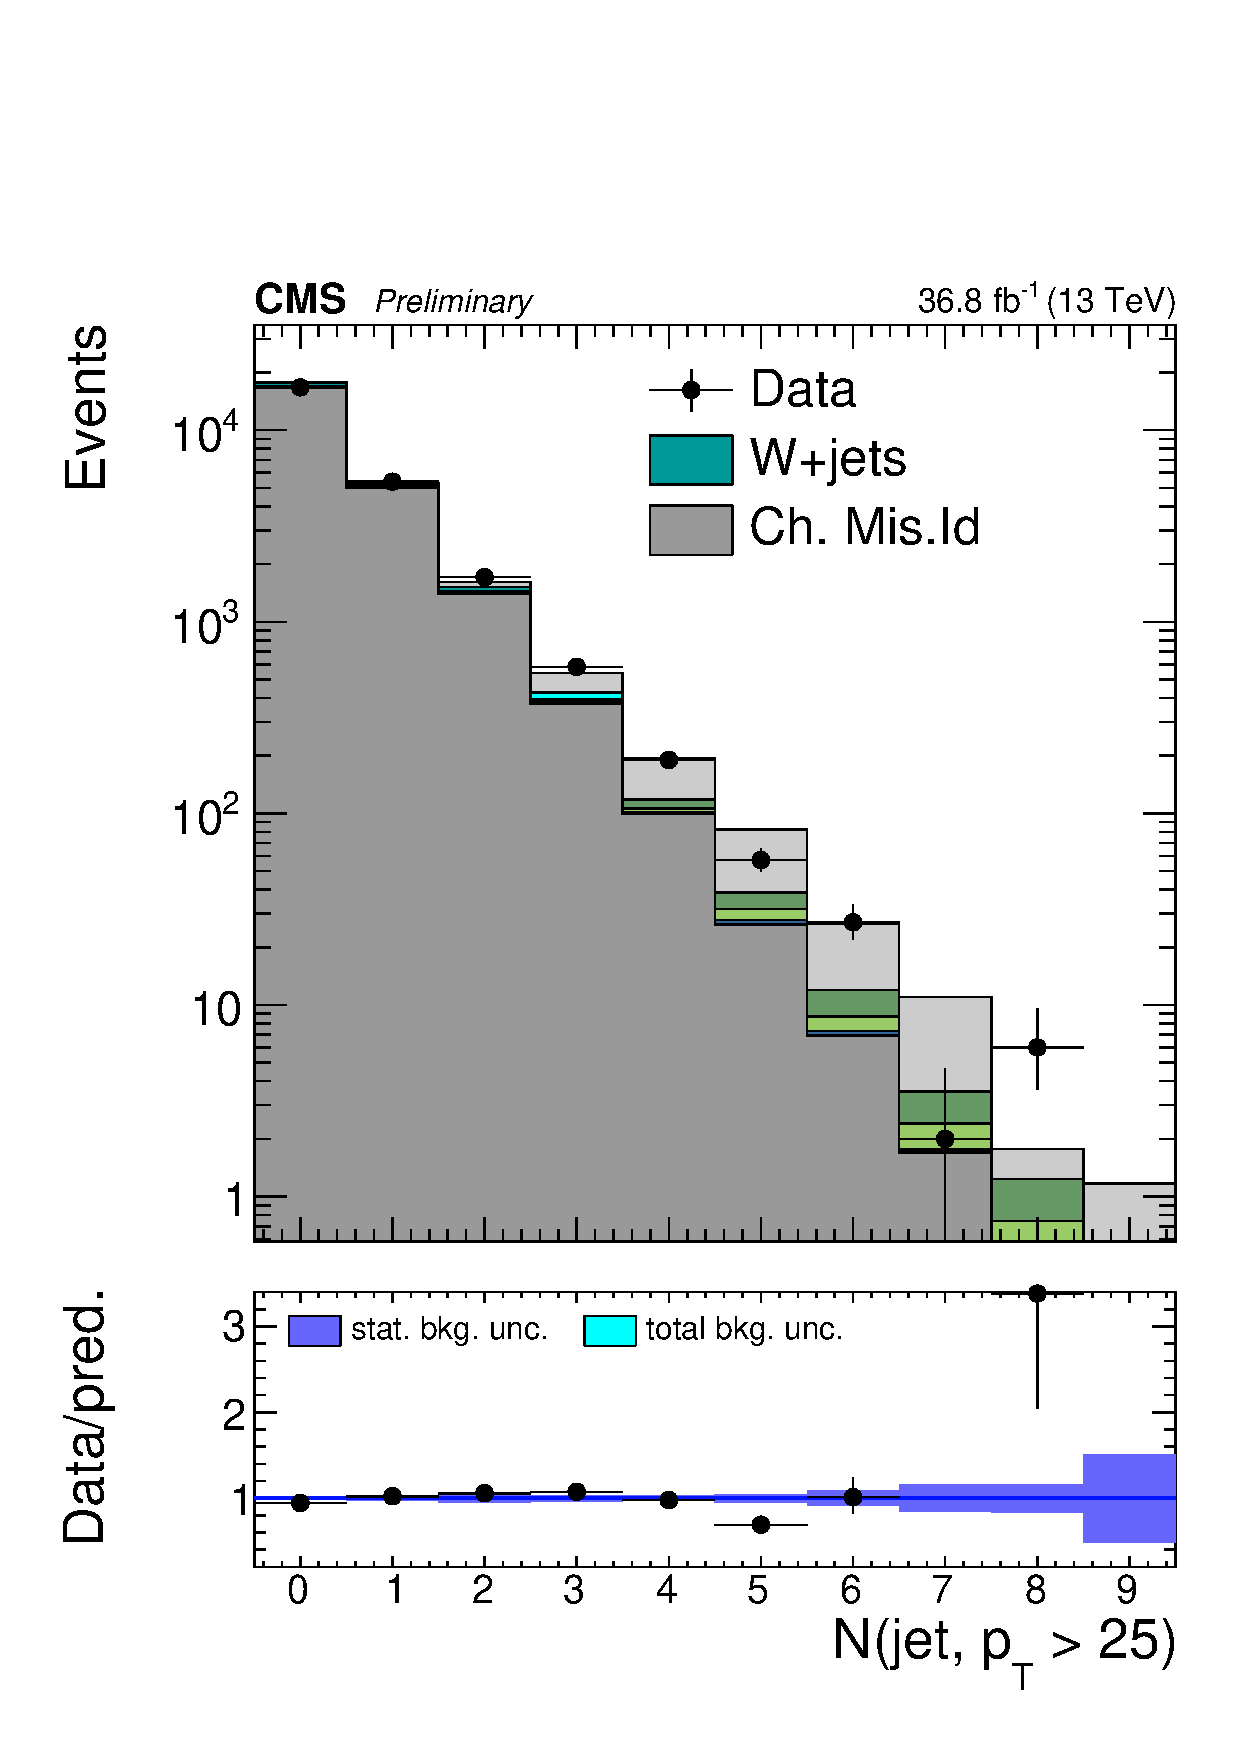
\includegraphics[width=0.32\textwidth]{plots_leptons/chargeflip/closure_dy/nJet25.pdf}
	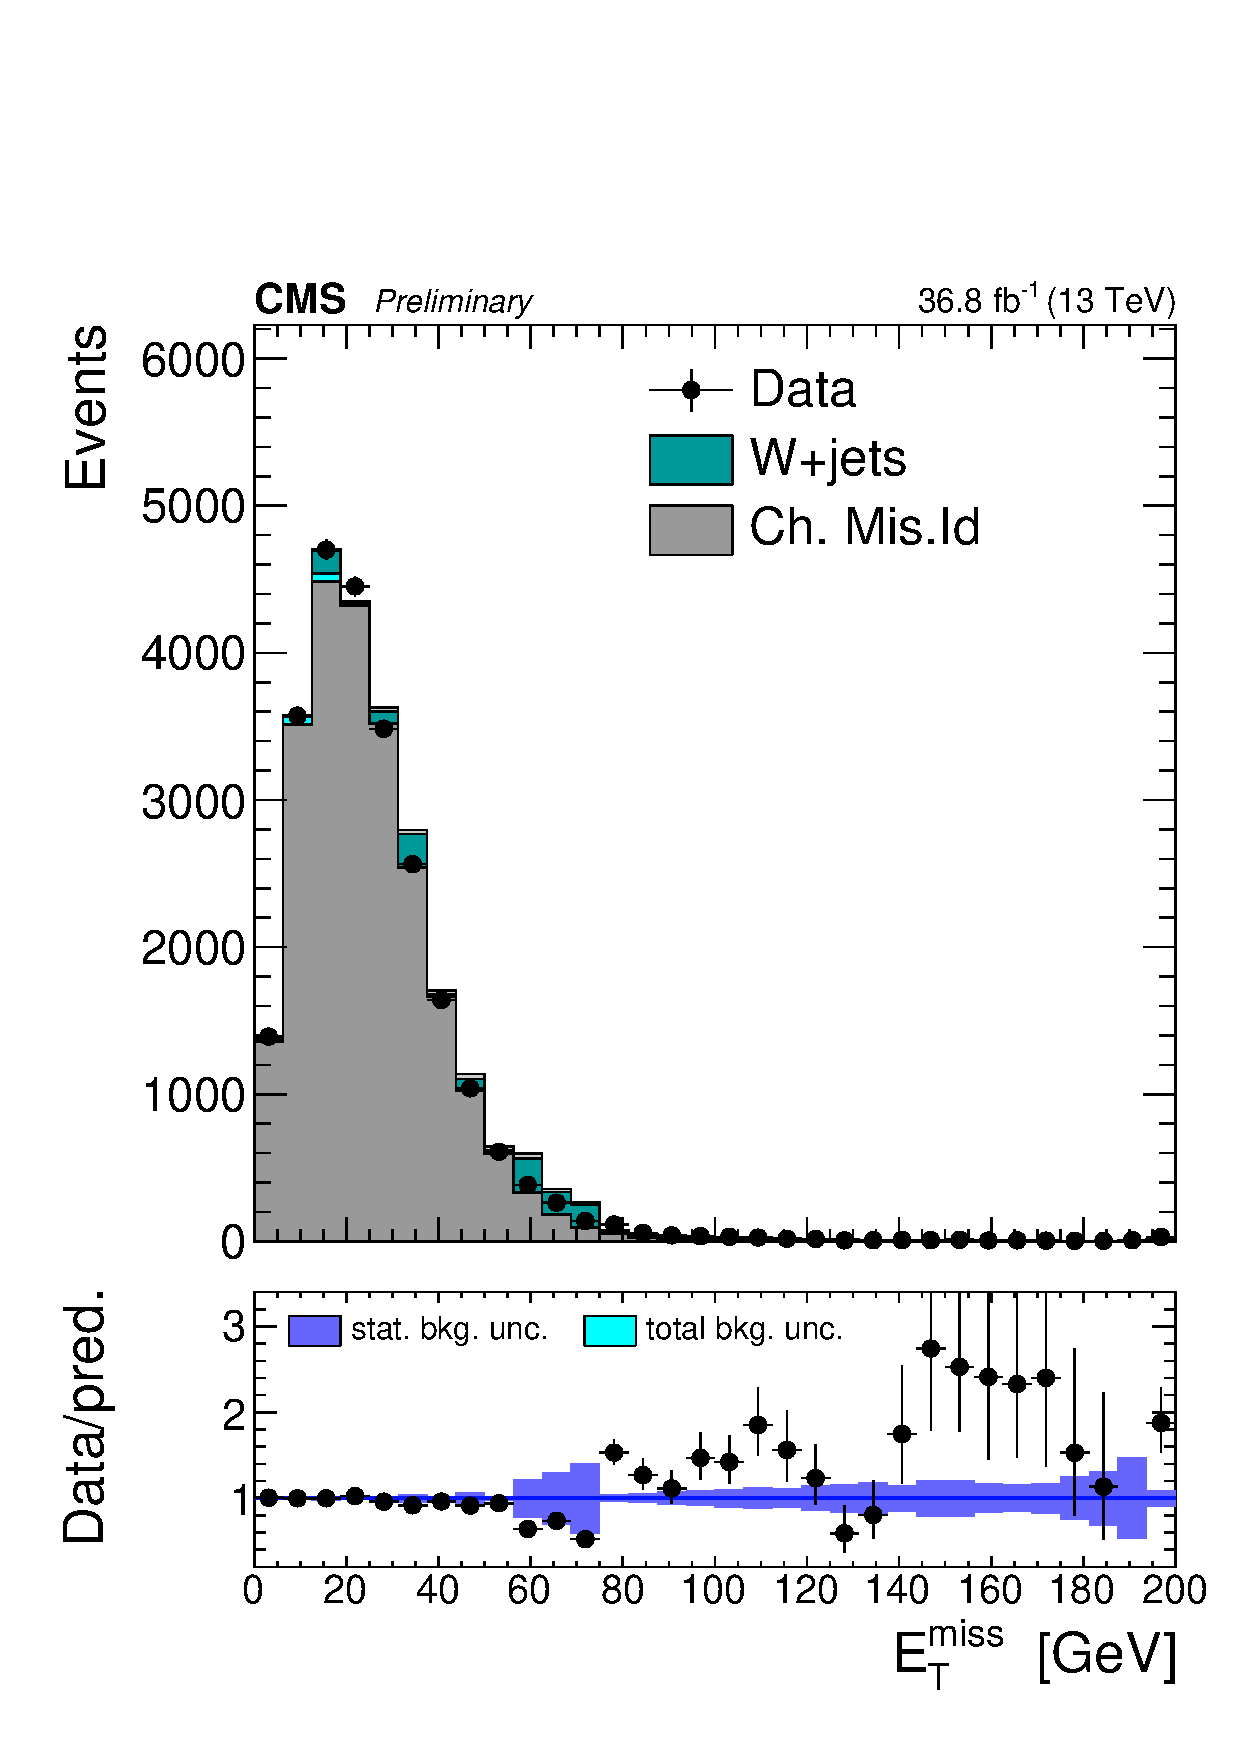
\includegraphics[width=0.32\textwidth]{plots_leptons/chargeflip/closure_dy/met.pdf}
	\caption{
	Charge misassignment closure test in DY dominated control region (where the misassignment probabilities are extracted from).
	}
	\label{fig:chmisid_closure_dy}
\end{figure}

\begin{figure}[htp]
	\centering
	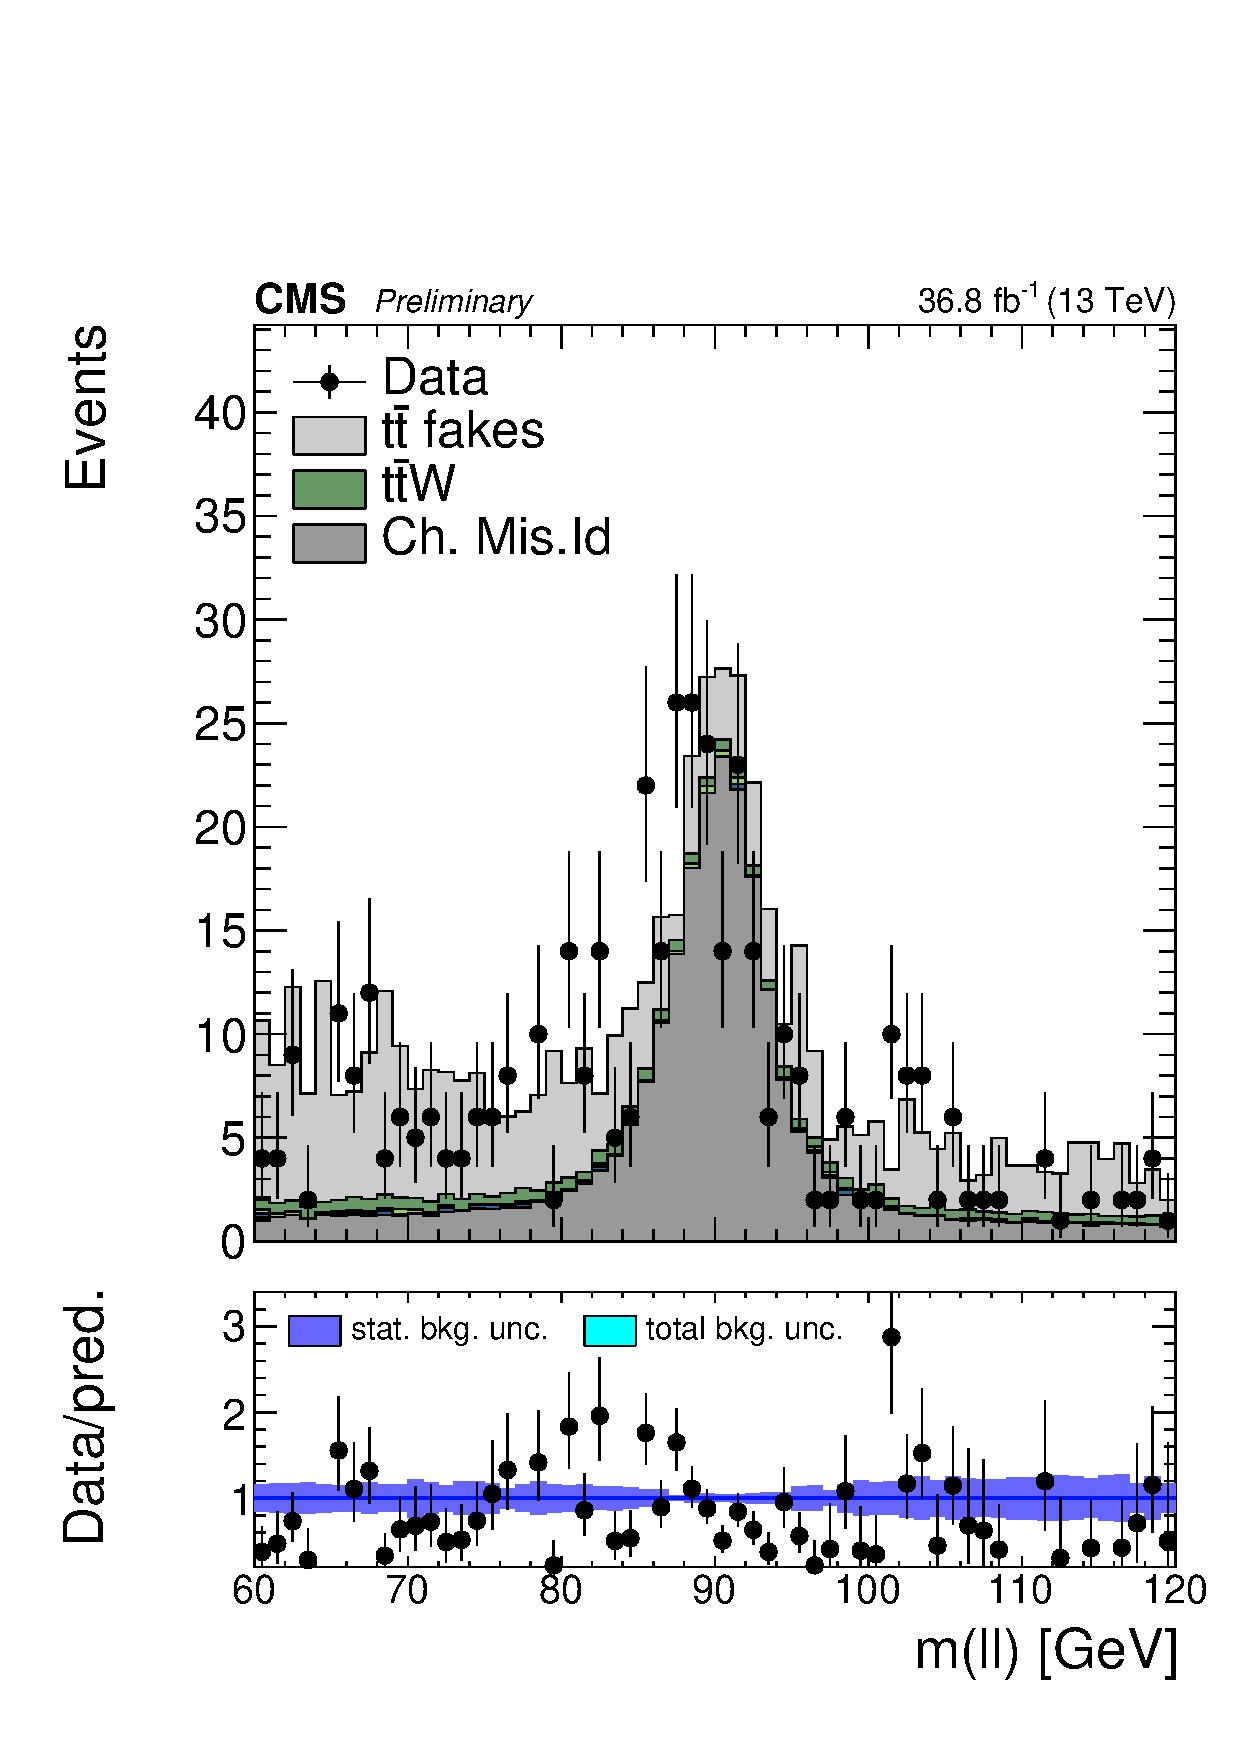
\includegraphics[width=0.32\textwidth]{plots_leptons/chargeflip/closure_tt/minMllAFAS.pdf}
	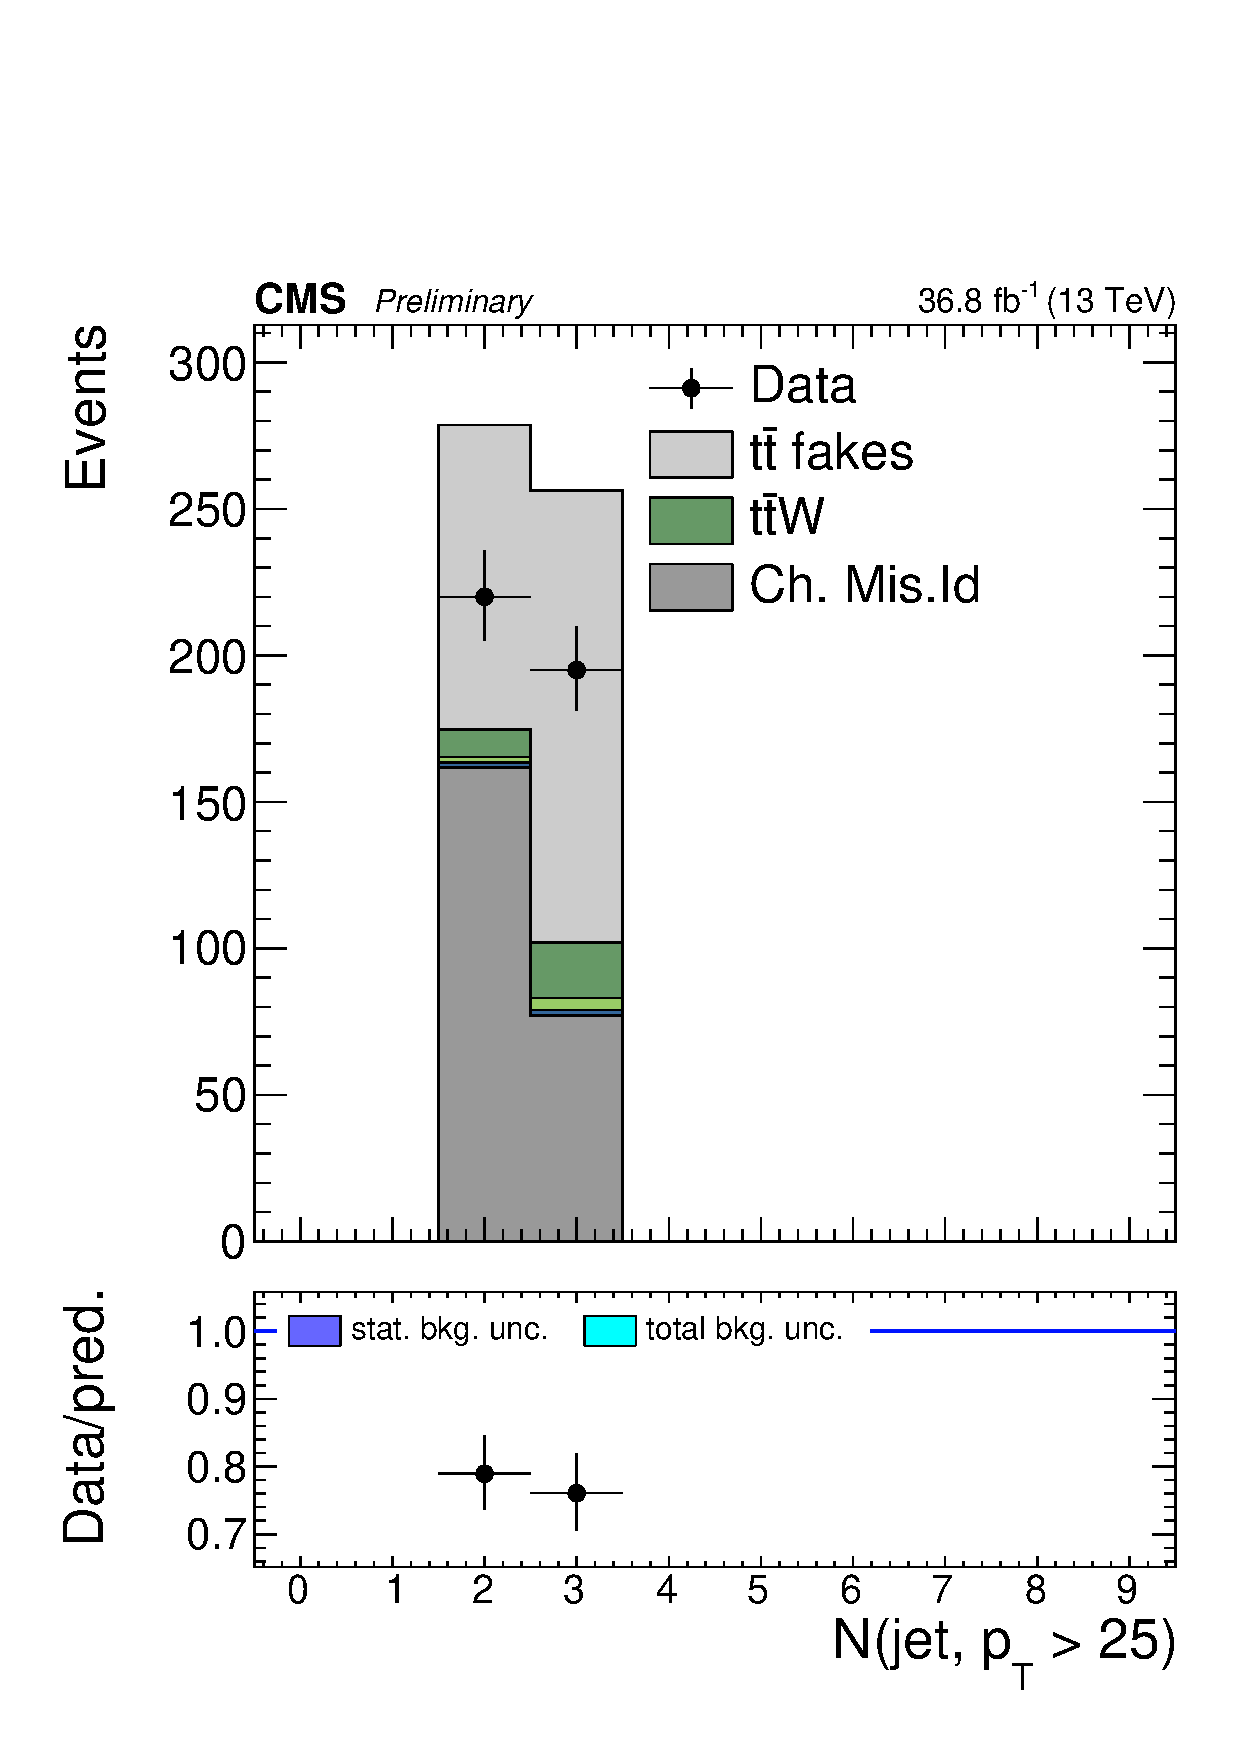
\includegraphics[width=0.32\textwidth]{plots_leptons/chargeflip/closure_tt/nJet25.pdf}
	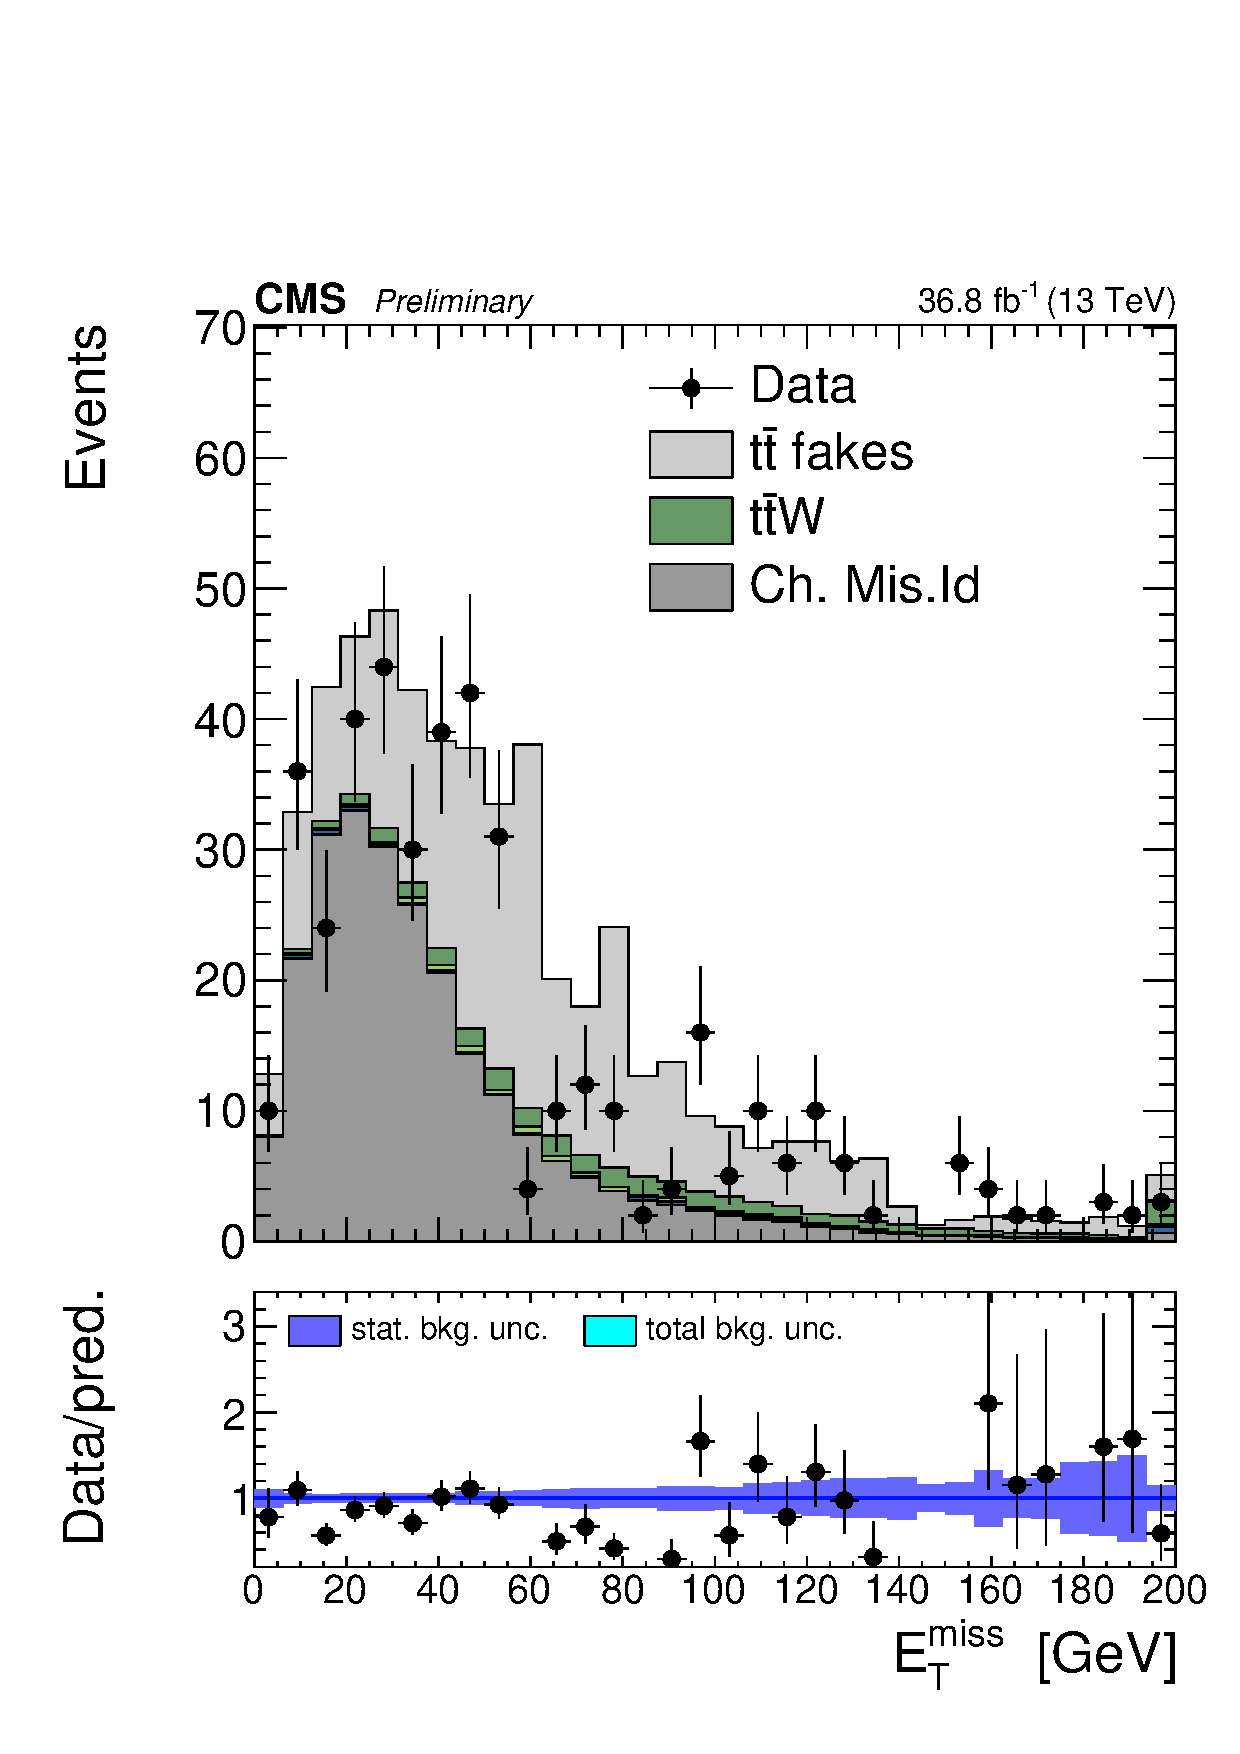
\includegraphics[width=0.32\textwidth]{plots_leptons/chargeflip/closure_tt/met.pdf}
	\caption{
	Charge misassignment closure test in a selection of exactly two same-sign electrons passing the full selection, between 2 and 3 hadronic jets, and at least one medium b-tagged jet or two loose b-tagged jets.
	}
	\label{fig:chmisid_closure_tt}
\end{figure}

From the statistical uncertainty of the measured probabilities and the good agreement of predicted charge-flip yields with the observed data distributions in the control regions, we assign a generous 30\% uncertainty on the predicted event yields from this background.

